\section{Tail mathematical model}
In order to devise a mathematical model of tail dynamics, we propose modeling the tail as a kinematic chain manipulator attached to robot body. Much like in aerial robots, when the robot is in the air, the tail acts freely on its body. We propose using the tail as a dynamic stabilization for the hopping. First we build the kinematic model using Denavit-Hartenberg parameterization method, after that we devise a dynamic model of the arms using recursive Newton-Euler algorithm.

\subsection{Kinematic model}
Kinematic chain of the tail is shown in Fig. \ref{fig:rmax}, and the kinematic parameters are shown in table \ref{tab:DHParameters}. Kinematic chain consists of the body coordinate system, 2 revolute joints  of the tail, one virtual prismatic joint in the tail (i.e. Tail length parameter), and the tail tip coordinate system. As can be seen from DH parameters table, the two revolute joints have no linear, only angular displacement from each other, therefore their masses and moments of inertia are all zero. The third prismatic joint represents the tail length and is modeled as a long stick with infitesimal thickness. 

\begin{table}
	\centering
		\begin{tabular}{ccccc}
		\hline
			& $\theta$ & $d$ & $a$ & $\alpha$ \\\hline
			\multicolumn{5}{c}{Body}\\\hline
			$B-0$ & $0$ & $d_B$ & $a_B$ & $0$\\\hline
			\multicolumn{5}{c}{Tail}\\\hline
			Joint 1 & $q_1$ & $0$ & $0$ & $-\frac{\pi}{2}$\\
			Joint 2 & $q_2$ & $0$ & $0$ & $\frac{\pi}{2}$\\
			Virtual joint& $0$ & $q_3$ & $0$ & $0$\\\hline
		\end{tabular}
	\caption{Denavit-Hartenberg Parameters}\label{tab:DHParameters}
\end{table}

\begin{equation}
T_0^3=\begin{bmatrix}
C_1 C_2 & -S_1 & C_1 S_2 & C_1 S_2 Q_3 \\
C_2 S_1 & C_1 & S_1 S_2 & S_1 S_2 Q_3 \\
-S_2 & 0 & C_2 & C_2 Q_3 \\
 0 & 0 & 0 & 1
\end{bmatrix}
\end{equation}

%\begin{multicols}{1}
\tiny
\begin{equation}
\tau_b=\begin{bmatrix}
\frac{1}{24} m_3 Q_3 \left(-12 g S_1 S_2+Q_3 \left(3 S_1 S2_2 {\dot{Q}_1}^2-2 C_1\left(5+3 C2_2\right) \dot{Q}_1 \dot{Q}_2-3 C_1 S2_2 \ddot{Q}_1-8 S_1 \ddot{Q}_2\right)\right)\\
\frac{1}{24} m_3 Q_3 \left(-12 g C_1 S_2+Q_3 \left(S_1\left( 2(5+3C2_2)\dot{Q}_1 \dot{Q}_2+3S2_2\ddot{Q}_1\right)+C_1(3S2_2{\dot{Q}_1}^2-8\ddot{Q}_2)\right)\right)\\
\frac{1}{4} S_2 m_3 Q_3^2 \left(2 C_2 \dot{Q}_1 \dot{Q}_2+S_2 \ddot{Q}_1\right)
\end{bmatrix}
\end{equation}
\normalsize
%\end{multicols}

\begin{figure}
	\centering
	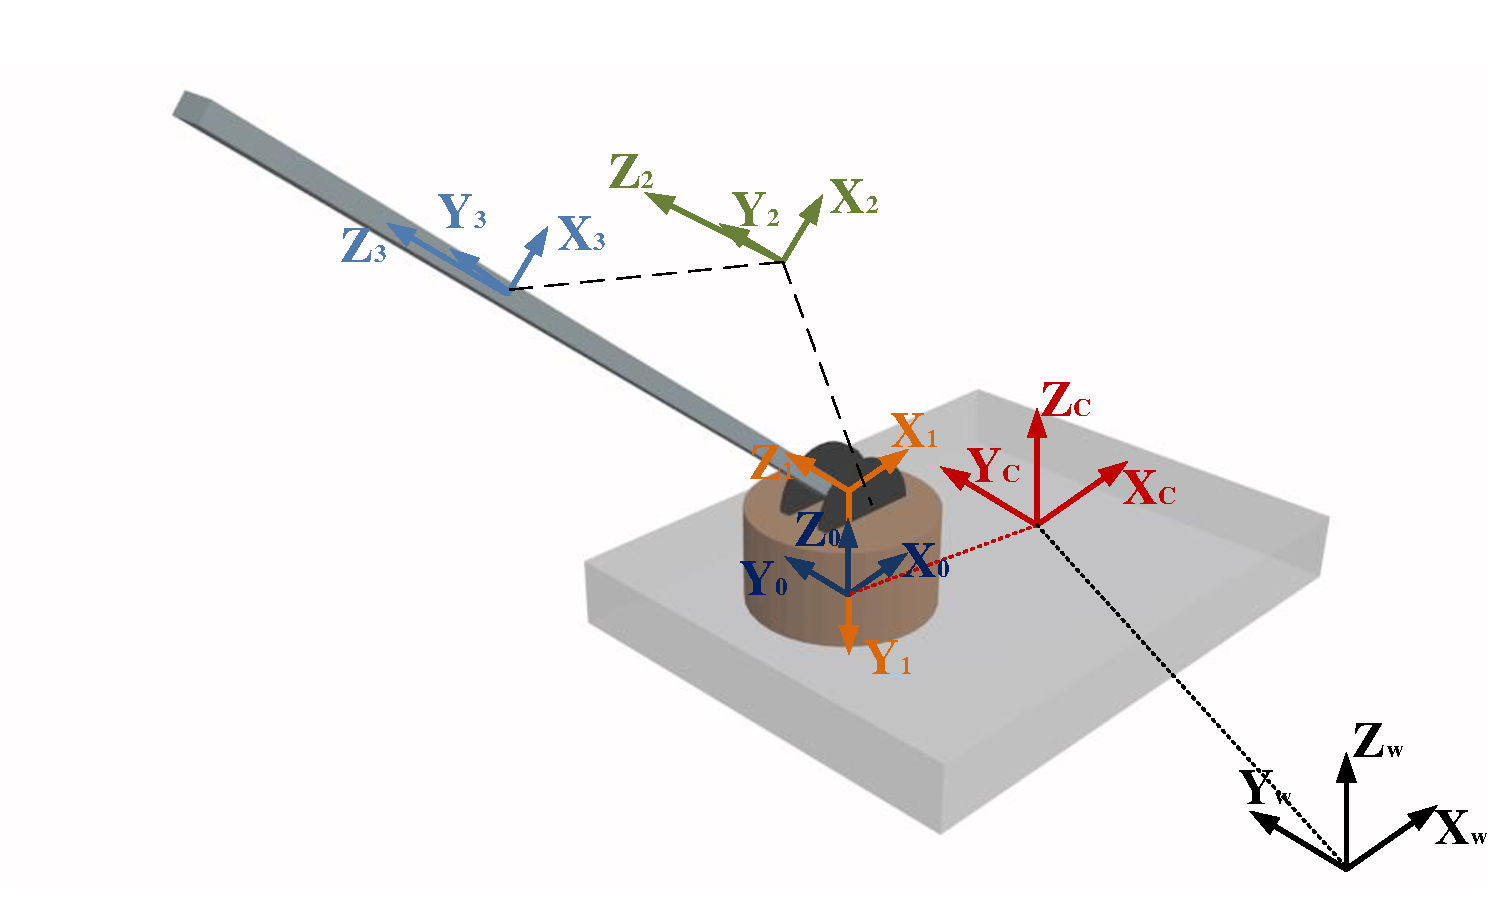
\includegraphics[width=85mm]{./pictures/RobinRepic.pdf}
	\caption{Robin Tail kinematic chain model}
	\label{fig:rmax}
\end{figure}

\subsection{Robin body}
In order to simplify the complexity of this analysis, we propose modeling Robin as a cuboid body, as shown in Fig \ref{fig:rmoment}. Moreover, Robin's body is a "container" for 4 cuboids, equally displaced from the body center. Ideally, when Robin's body is fully symmetric, all four cuboids have the same mass. Since in most situations this is not the case, each cuboid has its own mass $m_i$, its own center of mass $cm_i$ placed in its center, and $\vec{r}_i$, the distance between the $cm_i$ and the body coordinate system. The overall center of mass is then easily calculated from: 
\begin{equation}\label{eq:CMrobot}
CM=\frac{\sum_{i=1}^{4}m_i\vec{r}_i}{\sum_{i=1}^{4}m_i}
\end{equation}
Next important dynamic parameter is the moment of inertia tensor. Having for cuboid bodys as the basis of robot body model, tensor of inertia can easily be derived by using the Parallel axis theorem:

\begin{equation}
\tiny
J_R=\sum_{i=1}^{4}\left \{J_{c_i}+m_i\begin{bmatrix}
{_yr_i}^2+{_zr_i}^2 & {_xr_i}\cdot {_yr_i} & {_xr_i}\cdot {_zr_i} \\ 
-{_xr_i}\cdot {_yr_i} & {_xr_i}^2+{_zr_i}^2 & {_yr_i}\cdot {_zr_i}\\ 
-{_xr_i}\cdot {_zr_i} & {_yr_i}\cdot {_zr_i} & {_yr_i}^2+{_xr_i}^2
\end{bmatrix} \right \}
\normalsize
\end{equation}

where, $_xr_i, _yr_i, _zr_i$ represent $\vec{r}_i$ projection in $x,y,z$ respectively, and $J_{c_i}$ is the moment of inertia of the single cuboid element of height $h_i$, width $w_i$ and length $l_i$:
\begin{equation}
J_{c_i}=\frac{m_i}{12}\begin{bmatrix}
w_i^2+d_i^2 &0&0 \\ 
0 &h_i^2+d_i^2&0\\ 
0 &0& w_i^2+h_i^2
\end{bmatrix}
\end{equation} 

It could be easily shown that if all four cuboids have the same mass and size (i.e. $m,h,d,w$) and are symmetrically displaced from the body center, as shown in Fig \ref{fig:rmoment}, the total body moment of inertia $J_R$ comes down to a symmetric matrix: 
\begin{equation}
J_{c_i}=\frac{m}{12}\begin{bmatrix}
(2w)^2+d^2 &0&0 \\ 
0 &(2h)^2+d^2&0\\ 
0 &0& (2w)^2+(2h)^2
\end{bmatrix}
\end{equation} 
and the body center of mass is placed directly in the center of body coordinate system. For any other arrangement, tensor matrix will not be symmetric, and what is even worse, the body center of mass will be misaligned.

Acting as an active spring, while quadruped is hoping, each leg exerts force on its body. The legs are positioned symmetrically around the geometric center, and similarly as quadrotor aircraft produce the following forces and torques:

\begin{gather}\label{eq:Forces}
\vec{F_{tot}}=\sum_{i=1}^{4}(\vec{T_{i}}+\vec{S_{i}})\\
\vec{\tau_{tot}}=\sum_{i=1}^{4}\vec{\rho _i}\times(\vec{T_{i}}+\vec{S_{i}})
\end{gather}  

Where $\vec{T_{i}}$ represents the $i$-th cuboid thrust force that causes vertical movement (i.e. hopping), $\vec{S_{i}}$ $i$-th cuboid side force that moves the quadruped in x direction, and $\rho _i$ $i$-th distance between the geometric center and the forces.

\begin{figure}
	\centering
	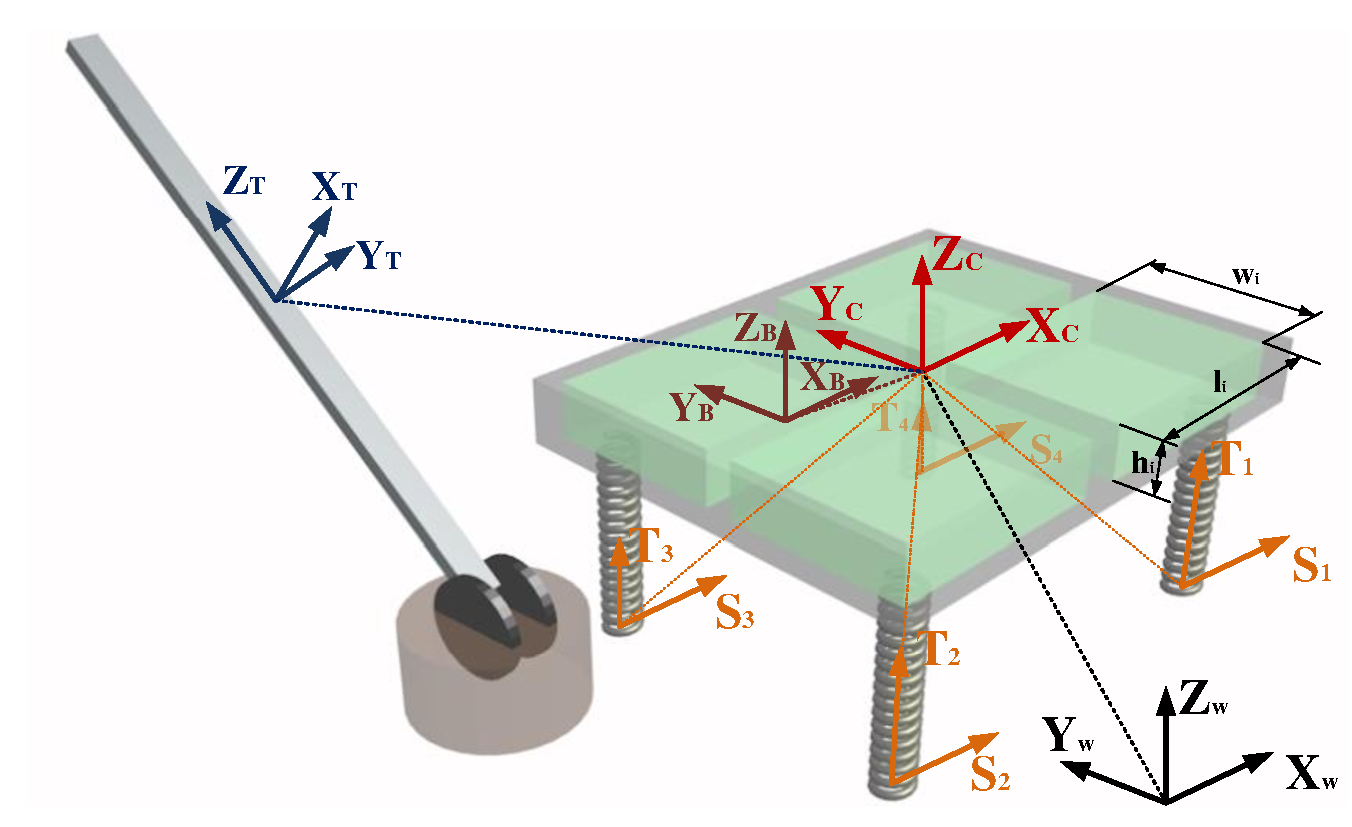
\includegraphics[width=85mm]{./pictures/RobinMoment.pdf}
	\caption{Robin body dynamics}
	\label{fig:rmoment}
\end{figure}

For a perfect symmetric body follows that the total torque (\ref{eq:Forces}) acting on the body is equal to zero, and the total force is the sum of all 4 active springs. For this, the necessary condition is that all four springs have exactly the same parameters, and thus exert the same forces. In reality, neither the springs are the same, nor there can be a perfectly symmetric body. We write the body torque equation for a non-symmetric body, with the center of mass displaced for $\vec{\Delta CM}$:

\begin{equation}\label{eq:Torques}
\vec{\tau}_{tot}=\begin{bmatrix}
\Delta \textsc{cm}_y \:\bar{T} & -\left ( \Delta \textsc{cm}_x \:\bar{T} +\Delta \textsc{cm}_z \:\bar{S}\right ) & -\Delta \textsc{cm}_y \:\bar{S}
\end{bmatrix}^T
\end{equation}
where $\bar{T}$ and $\bar{S}$ represent the average thrust and side forces of each leg. In this analysis, the displacement of the center of mass is used to model the unbalanced body dynamics. In practice, the displacement vector  $\vec{\Delta CM}$ can incorporate all possible imperfections: design symmetry, leg differences, motor dynamics and so on.  

In order to achieve successful hopping average forces $\bar{T}$ and $\bar{S}$ have to exist. On the other hand, for a stable jump, we need to counteract the undesired torque (\ref{eq:Torques}). Therefore, we propose, adding a tail to the quadruped in order to balance the robot. 
\subsection{Tail dynamics}
In Fig. \ref{fig:rmoment}, a tail with its ${L_T}$ coordinate system, placed in its center of mass is depicted. Introducing a new body in the quadruped construction, the overall center of mass will change accordingly:
\begin{equation}\label{eq:CMrobotAndTail}
CM=\frac{\sum_{i=1}^{4}m_i\vec{r}_i+m_T\vec{p}_T}{\sum_{i=1}^{4}m_i+m_T}= \frac{\Delta\vec{\textsc{cm}}+\mu\cdot\textsc{cm}_T}{1+\mu}
\end{equation}
In the previous equation we introduced the mass ratio $\mu=\frac{m_T}{\sum_{i=1}^{4}m_i}$ and $\Delta\vec{\textsc{cm}}$ is the center of mass of the robot without the tail from equation (\ref{eq:CMrobot}). If we want to keep the center of mass in the construction center of the robot (i.e. $CM=0$), then the following condition has to be met:
\begin{equation}\label{eq:CMzeroing}
\begin{bmatrix}
\Delta \textsc{cm}_x\\ 
\Delta \textsc{cm}_y\\ 
\Delta \textsc{cm}_z
\end{bmatrix}+
\frac{\mu Q_3}{2}\begin{bmatrix}
C_1S_2\\ 
S_1S_2\\ 
C_2
\end{bmatrix}=0
\end{equation}
that is to say, that the numerator in (\ref{eq:CMrobotAndTail}) has to be zero. Given that in (\ref{eq:CMzeroing}) there exists only two variables, $Q_1$ and $Q_2$ respectively, one can eliminate only two components of center of mass displacement vector $\Delta \vec{\textsc{cm}}$. Under a reasonable assumption that $\bar{T}\gg \bar{S}$, from equation (\ref{eq:Torques}) follows that for a stable jump one needs to successfully eliminate $x$ and $y$ components of center of mass displacement vector. This assumption is reasonable because in most cases the forward motion is slow compared to the jumping action, and in z direction one needs to overcome the gravity acceleration $g$, making $\bar{T}$ by the order of magnitude larger then $\bar{S}$.

From a strict mathematical point of view, the necessary condition for (\ref{eq:CMzeroing}) to have a solution is:
\begin{equation}\label{eq:CMcondition}
\frac{\mu Q_3}{2}\geq \textup{MAX}\left \{ \left | \Delta \textsc{cm}_x \right |, \left | \Delta \textsc{cm}_y \right |,\left | \Delta \textsc{cm}_z \right |\right \}
\end{equation}
When the condtion (\ref{eq:CMcondition}) is met, the analytical solution to equation (\ref{eq:CMzeroing}) can easily be derived:
\begin{gather}\label{eq:CMsolution}
Q_1=atan2\left({\Delta \textsc{cm}_y},\, {\Delta \textsc{cm}_x}\right)\\
Q_2=asin\left(\frac{2\sqrt{{\Delta \textsc{cm}_x}^2+{\Delta \textsc{cm}_y}^2}}{\mu Q_3} \right)
\end{gather}

\subsubsection{Iterative Center of Mass displacement compensation}
In reality, the distribution of center of mass of the body is not known, and therefore, analytic solution give with (\ref{eq:CMsolution}) is impossible. Thus an iterative method, based on hopping response is proposed. When a quadruped is hopping, its contact with the ground is infitesimally short, and consequently, reaction forces and torques are approximated with the Dirac function $\delta (s)$. During the jump, the body behaves according to Euler body dynamics function (\ref{eq:EulerBody}). Taking account the infitessimally short time the body has to accelerate the cross coupling term $\vec{\omega}\times J_B\vec{\omega}$ can be neglected and the rotation speed vector can be approximated with (\ref{eq:RotSpeedAprox}).
\begin{figure}
	\centering
	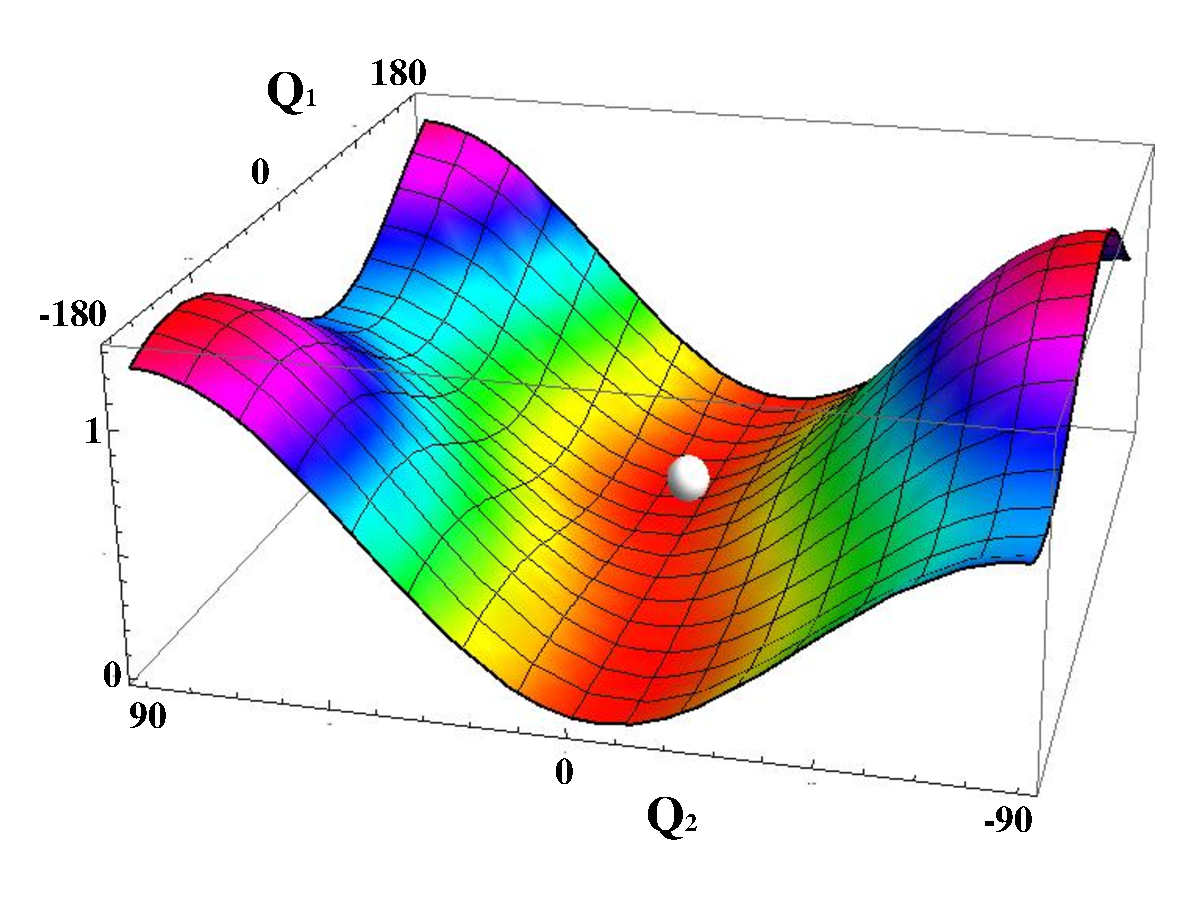
\includegraphics[width=85mm]{./pictures/RobinRepicCM.pdf}
	\caption{Center of mass displacement}
	\label{fig:rmoment}
\end{figure}

\begin{equation}\label{eq:EulerBody}
\tau_{tot}=J_B\vec{\dot{\omega}}+\vec{\omega}\times J_B\vec{\omega}
\end{equation}

\begin{equation}\label{eq:RotSpeedAprox}
\vec{\omega}\approx \frac{1}{s}{J_B}^{-1}\begin{bmatrix}
\Delta \textsc{cm}_y & -\Delta \textsc{cm}_x & 0
\end{bmatrix}^T\bar{T}\delta(s)
\end{equation}

Calculating the distance of vector (\ref{eq:RotSpeedAprox}) it is easy to show how the size of rotation speed vector is proportional to the displacement of center of mass. This effectively shows how moving the displacement of center of mass to the construction center of the robot eliminates the generation of unwanted rotations. 

\begin{equation}
\left \| \vec{\omega} \right \|\sim \sqrt{{\Delta \textsc{cm}_x}^2+{\Delta \textsc{cm}_y}^2}
\end{equation}


In order to iteratively calculate the angles $q1$ and $q2$, angular velocity vector is recorded during start of hopping acceleration phase $F_1$. This phase lasts until one of the leg/spring reaches desired length $L_d$. The leg which carries a minimum mass will achieve the fastest acceleration and the algorithm task is to navigate tail towards this leg. 

For example, mass distribution in figure  (\ref{fig:imassCom}) is equally distributed except for $MASS_2$  which is lighter then others. At the end of phase $F_1$ the body rotates at an angular velocity $\vec{\omega}$. By using the cross product of projection vector $\vec{\omega_{xy}}$ in $XY$ plane and body $\vec{Zb}$, the tail direction vector $\vec{\omega_{TD}}$ is calculated. 

Tail motion control algorithm navigates tail in vector $\vec{\omega_{TD}}$ direction which at the end results the equal mass distribution.

\begin{figure}
	\centering
	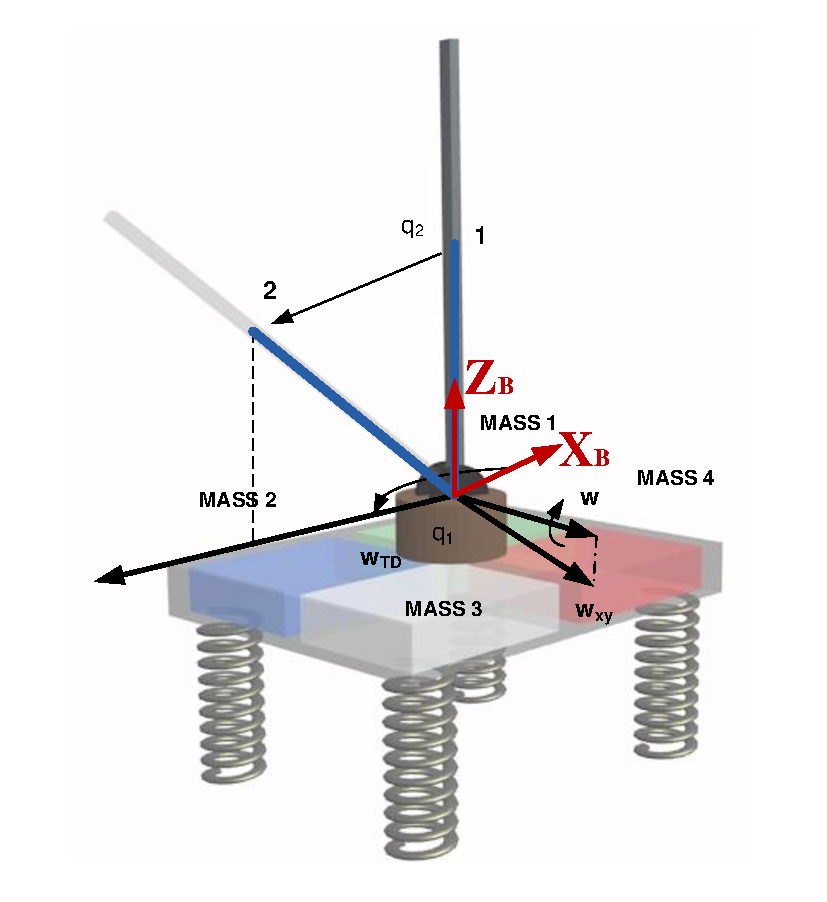
\includegraphics[width=85mm]{./pictures/IterativeAlgorithm.pdf}
	\caption{Iterative mass displacement compensation}
	\label{fig:imassCom}
\end{figure}





Due to the tail's infitesimal thickness, its moment of inertia, written in this frame can be simplified:
\begin{equation}
J_T=J_3=\frac{{Q_3}^2 m_3}{12}\left(
\begin{array}{ccc}
 1 & 0 & 0 \\
 0 & 1 & 0 \\
 0 & 0 & 0
\end{array}
\right)
\end{equation} 
\small
\begin{equation}
{J_T}^*={R_0^3}^TJ_TR_0^3+m_T\begin{bmatrix}
{cm_y^T}^2 +{cm_z^T}^2& {cm_x^T}{cm_y^T}& {cm_x^T}{cm_z^T} \\ 
-{cm_x^T}{cm_y^T} & {cm_x^T}^2+{cm_z^T}^2 & {cm_y^T}{cm_z^T}\\ 
-{cm_x^T}{cm_z^T} & -{cm_y^T}{cm_z^T} & {cm_x^T}^2+{cm_y^T}^2
\end{bmatrix}
\end{equation}
\normalsize
